% !TEX TS-program = pdflatex
% !TEX encoding = UTF-8 Unicode

% This is a simple template for a LaTeX document using the "article" class.
% See "book", "report", "letter" for other types of document.

\documentclass[10pt]{article} % use larger type; default would be 10pt
\usepackage{color}
\usepackage[utf8]{inputenc} % set input encoding (not needed with XeLaTeX)

%%% Examples of Article customizations
% These packages are optional, depending whether you want the features they provide.
% See the LaTeX Companion or other references for full information.

%%% PAGE DIMENSIONS

% \geometry{margins=2in} % for example, change the margins to 2 inches all roudn
% \geometry{landscape} % set up the page for landscape
%   read geometry.pdf for detailed page layout information

\usepackage{graphicx} % support the \includegraphics command and options

% \usepackage[parfill]{parskip} % Activate to begin paragraphs with an empty line rather than an indent

%%% PACKAGES
\usepackage{booktabs} % for much better looking tables
\usepackage{array} % for better arrays (eg matrices) in maths
%\usepackage{paralist} % very flexible & customisable lists (eg. enumerate/itemize, etc.)

%\usepackage{subfig} % make it possible to include more than one captioned figure/table in a single float
\usepackage{amsfonts}
\usepackage{amsthm}
\usepackage{tikz}
%\SetVertexNormal[Shape     = circle, LineWidth = 2pt]
%\SetUpEdge[lw    = 1.5pt, color = blue]
\usepackage{amsmath}
\usepackage{float}
\usepackage{graphicx}
\usepackage{caption}
\usepackage{subcaption}
\usepackage{color}
\usepackage{amssymb}
\usepackage{bm}

% These packages are all incorporated in the memoir class to one degree or another...

%%% HEADERS & FOOTERS
\usepackage{fancyhdr} % This should be set AFTER setting up the page geometry
\pagestyle{fancy} % options: empty , plain , fancy
\renewcommand{\headrulewidth}{0pt} % customise the layout...
\lhead{}\chead{}\rhead{}
\lfoot{}\cfoot{\thepage}\rfoot{}

%%% SECTION TITLE APPEARANCE
%\usepackage{sectsty}
%\allsectionsfont{\sffamily\mdseries\upshape} % (See the fntguide.pdf for font help)
% (This matches ConTeXt defaults)

%%% ToC (table of contents) APPEARANCE
%\usepackage[nottoc,notlof,notlot]{tocbibind} % Put the bibliography in the ToC
%\usepackage[titles,subfigure]{tocloft} % Alter the style of the Table of Contents
%\renewcommand{\cftsecfont}{\rmfamily\mdseries\upshape}
%\renewcommand{\cftsecpagefont}{\rmfamily\mdseries\upshape} % No bold!


\newtheorem{theorem}{Theorem} 
\newtheorem{lemma}{Lemma}
\newtheorem{propn}{Proposition}
\newtheorem*{thmm}{Theorem}
\newtheorem{remk}{Remark} 
\newtheorem{corol}{Corollary}
\newtheorem{definition}{Definition}
\newtheorem{ques}{Question}


\newtheorem{thm}{Theorem}[section] 
\newtheorem{prop}[thm]{Proposition} 
\newtheorem{lem}[thm]{Lemma}
\newtheorem{cor}[thm]{Corollary} 
\newtheorem{con}[thm]{Conjecture} 

\theoremstyle{definition}
\newtheorem{defn}[thm]{Definition}
\newtheorem*{rem}{Remark}
%\newtheorem*{nota}{Notation}
\newtheorem*{nota}{Notation}
\newtheorem{cla}[thm]{Claim}
\newtheorem{ex}[thm]{Example}
\newtheorem{exs}[thm]{Examples}
\newtheorem*{exer}{Exercise}
\newtheorem{case}{Case}
\newtheorem{conj}{Conjecture}


\definecolor{sotonblue}{rgb}{0.0,0.394,0.597}
\DeclareMathOperator{\Pos}{Pos}
\DeclareMathOperator{\p}{\text{Pr\"{u}fer}}
\DeclareMathOperator{\m}{m}
%\DeclareMathOperator{\deg}{deg}

%opening
 \title{Prufer sequences}
\author{David Matthews}
\begin{document}


\section{Introduction}
Cayley was first to prove that there are $n^{n-2}$ labeled, rooted trees on $n$ vertices \cite{Cayley}. A later proof due to Pr\"{u}fer uses a correspondence between particular sequences called \emph{Pr\"{u}fer sequences} and labeled trees \cite{Bela}.  

In Section \ref{ps} we will characterize the subset of Pr\"{u}fer sequences that correspond to a family of trees called \emph{increasing trees}.   
%Random recursive trees. 

\section{Pr\"{u}fer Sequences}\label{ps}

\subsection{Notation}
For succinctness we will use $\mathbb{N}_{n}:= \{1,2,3,\dots,n\}$ and by \emph{tree} we mean labelled, rooted, non embedded tree throughout this section.  If $A$ and $B$ are sequences we say that $A \backslash B$ consists of all the distinct entries of $A$ that are not in $B$.  Given some graph $G$ we denote $V(G)$ to be set of vertices of $G$ and we say that $E(G)$ is the set of edges of $G$.  If $v,w \in V(G)$ and there is a edge, $e \in E(G)$, joining $v$ and $w$ then we write $e = (v,w)$ amd say that $v$ is connected via an edge to $w$.  Given some $v \in V(G)$ the degree of $v$ is denoted $\deg(v)$ and we say that vertices $v$ such that $\deg(v) = 1$ are \emph{leaves}.   A tree is an \emph{increasing tree} if every vertex other than the root is adjacent to precisely one other vertex with a lower label.  Note that we will write a vertex $i$ interchangeably with a vertex labelled $i$ throughout.

\subsection{The Pr\"{u}fer Correspondence}

Any sequence $P_{n} = (a[1],a[2],\dots,[n-2])$ such that every $a[i] \in \mathbb{N}_{n}$ is a Pr\"{u}fer sequence.  For example the following sequence is a valid Pr\"{u}fer sequence:
\[P_{10} = (4,3,2,8,1,1,2,4).\]
We will use the notation $P_{n}[i:j]$ to mean the $i^{th} - j^{th}$ entries (inclusive) of a given Pr\"{u}fer sequence. In terms of the example above $P_{10}[3 : 7] = (2,8,1,1,2)$. We define $P_{n}[x:y]$ to be the empty sequence if $y < x $.  

Let $X_{v}$ denote the multiplicity of the label $v$ in $P_{n}$.  For example, if we consider $P_{10}$ defined above: 
\[X_{1}=2,\text{  } X_{2}=2,\text{  } X_{3}=1,\text{   } X_{4} = 2, \text{   } X_{5} = 0 \dots\]
Given some Pr\"{u}fer sequence $P_{n}$ we can associate  a sequence 
\[\Pos_{v} = (\Pos_{v,1},\Pos_{v,2},\dots,\Pos_{v,X_{v}})\]
to every $v \in P_{n}$ such that $\Pos_{v,j}$ is the position of the $j^{th}$ occurrence of $v$. For example, entry $4$ occurs in the first and eighth position of $P_{10}$ so $\Pos_{4} = (1,8)$.  For any $v \in P_{n}$ we say that an occurrence of $v$ is \emph{final} if that occurrence of $v$ is in position $\Pos_{v,X_{v}}$. We define $L = \{ v : v \in \mathbb{N}_{n} \backslash P_{n}\}$. In our example $L = \{5,6,7,9,10\}$.

We can associate a tree witha Pr\"{u}fer sequence $P_{n} = (a[1],a[2],\dots,a[n-2])$ via a dynamic correspondence. At each time, $t$ an appropriate vertex is chosen from a set of available vertices and is attached via an edge to $a[i]$.   At time $t = 0$ set $L_{0} = L$ and define $G_{0}$ to be the graph on $n$ vertices labelled $1,2,\dots,n$ with no edges. At time $t=1$ the vertex with label $a[1]$ is attached via an edge to $\min L_{0}$ to form $G_{1}$.  More generally, at time $t$ we form $L_{t}$ from $L_{t-1}$ by removing $\min L_{t-1}$ and adding $a[t-1]$ if $a[t-1]$ is final and form $G_{t}$ by connecting via an edge the labelled vertex $a[t]$ to vertex $\min L_{t}$ for $t = 2,3,4,\dots,n-2$.  Let $D$ be the number of distinct entries of $P_{n}$. Since $D$ elements are added to $L_{0}$ and $n-2$ elements are removed to form $L_{t-1}$:
\[|L_{n-1}| = |L_{0}| + D - (n-2).\]
Clearly $D + |L_{0}| = n$ therefore $|L_{n-1}| = 2$. Finally, $G_{n-1}$ is formed by adding an edge between these vertices.

It is known that $G_{n-1}$ is always a tree on $n$ nodes so we write $T_{n}:=G_{n-1}$.  It is also known that $\deg(v) = X_{v} + 1$ for all $v \in V(T_{n})$. Therefore $L$ corresponds to the leaves of $T_{n}$.  %At time $t$ the vertices $v \in L_{t}$ are said to be \emph{available} for attachment.  

\begin{ex}
Let $P = (4,3,2,8,1,1,2,4)$. We build the corresponding tree, $T$, as follows.  Let $G_{0}$ be the graph on 10 vertices with 0 edges.  At time $t=0$ $L_{0} = L =  \{5,6,7,9,10\}$ therefore we build $G_{1}$ from $G_{0}$ by adding an edge between the vertex labelled 4 and the vertex labelled $\min L_{0} = 5$. Since $4$ is not final $L_{1} = \{6,7,9,10\}$ and we build $G_{2}$ by adding edge $(3,6)$ to $G_{1}$.  Since 3 is final $L_{2} = \{3,7,9,10\}$ so we form $G_{3}$ by adding the edge $(2,3)$ to $G_{2}$.  This process continues until we build $T_{n}$ shown in Figure \ref{fig:1}:

\begin{figure}
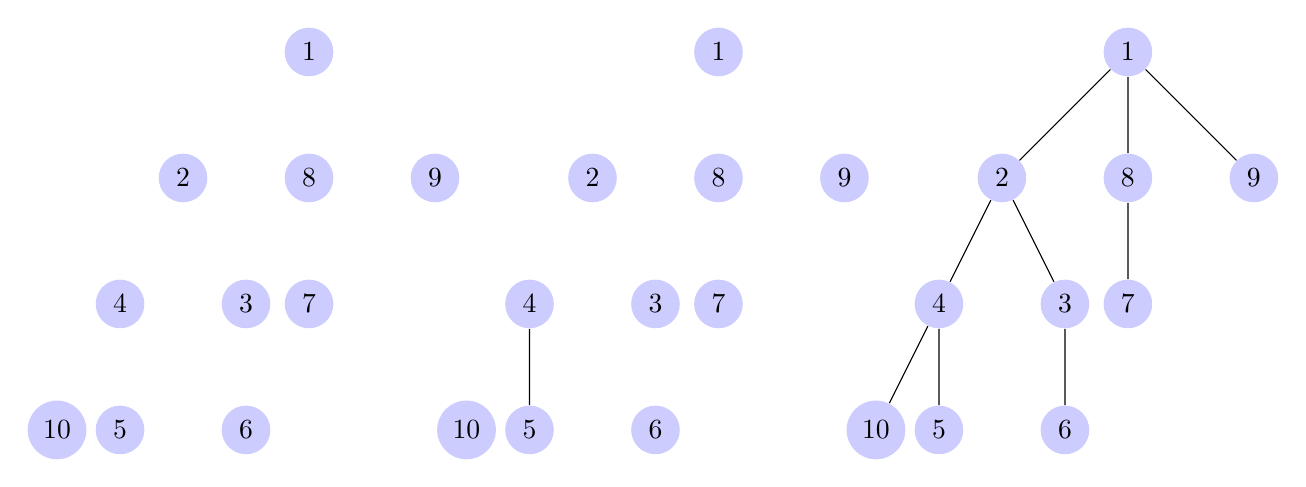
\begin{tikzpicture}
  [scale=.8,auto=left,every node/.style={circle,fill=blue!20}]
 \tikzset{EdgeStyle/.style={->}}
  
  \node (n11) at (4,8) {1};
 \node (n12) at (2,6)  {2};
  \node (n13) at (3,4)  {3};
 \node (n14) at (1,4) {4};
  \node (n15) at (1,2)  {5};
  \node (n16) at (3,2)  {6};
  \node (n17) at (4,4)  {7};
  \node (n18) at (4,6)  {8};
 \node (n19) at (6,6)  {9};
 \node (n20) at (0,2) {10};
  
  \node (n21) at (10.5,8) {1};
 \node (n22) at (8.5,6)  {2};
  \node (n23) at (9.5,4)  {3};
 \node (n24) at (7.5,4) {4};
  \node (n25) at (7.5,2)  {5};
  \node (n26) at (9.5,2)  {6};
  \node (n27) at (10.5,4)  {7};
  \node (n28) at (10.5,6)  {8};
 \node (n29) at (12.5,6)  {9};
 \node (n30) at (6.5,2) {10};
  
  \node (n1) at (17,8) {1};
  \node (n2) at (15,6)  {2};
  \node (n3) at (16,4)  {3};
  \node (n4) at (14,4) {4};
  \node (n5) at (14,2)  {5};
  \node (n6) at (16,2)  {6};
  \node (n7) at (17,4)  {7};
  \node (n8) at (17,6)  {8};
  \node (n9) at (19,6)  {9};
  \node (n10) at (13,2) {10};

 \foreach \from/\to in {n10/n4,n5/n4,n4/n2,n6/n3,n3/n2,n2/n1,n7/n8,n8/n1,n9/n1,n24/n25}
    \draw (\from) -- (\to);

\end{tikzpicture}
\caption{$G_{0}$ is on the far left above.  $G_{1}$ is central above and $ T_{n} (=G_{n-1})$ is on the right above.}\label{fig:1}
\end{figure}

 \end{ex}

 \subsection{Increasing Trees}\label{sec:itr}
 
We can  associate another sequence $B_{n} = (b[1],b[2],\dots,b[n-2])$ of length $n-2$ with $P_{n}$ as follows:  firstly, for all $v \in P_{n}[1:n-3]$ we set $b[\Pos_{v,X_{v}} + 1] =  a[\Pos_{v,X_{v}}]$.

In our example: 
\[B_{10} = (\;,\;,3,\;,8,\;,1,2)\]
We then order $L$ from lowest to highest and fill the remaining empty entries of $B_{n}$ with the first $|L| - 1$ entries from $L$ ordered from lowest to highest.  For example,
\[B_{10} = (5,6,3,7,8,9,1,2)\] 
  
Let $m_{1} = \min P_{n}$.  If $1 \in P_{n}$ then $m_{1} = 1$.  If $1 \notin P_{n}$ then the vertex labelled 1 must be a leaf of $T_{n}$, if $n>2$ then the vertex labelled 2 cannot be a leaf so $m_{1} = 2$.   

We say that the (possibly empty) set $E = \{e_{1},e_{2},\dots,e_{m}\}$ is the set  of \emph{ exceptional Pr\"{u}fer positions} ordered such that $e_{1} < e_2 <\dots <e_m$ and let $E$ be defined as follows.  

\begin{case}[$\min P_{n} = 1$] If $\Pos_{1,X_{1}} \neq n-2$ then $\Pos_{1,X_{1}} + 1 = e_1$ we then set $m_{2} = \min P_{n}[e_{1} : n-2]$ and if 
$\Pos_{m_{2}X_{m_{2}}} \neq n-2$ then $e_2 = \Pos_{m_{2}X_{m_{2}}}  + 1$.  In general $m_i = \min P_{n}[e_{i - 1} :n-2]$ and, if $\Pos_{m_{i}X_{m_{i}}} \neq 
n-2$ then $e_{i} = \Pos_{m_{i}X_{m_{i}}} + 1$.
\end{case}
\begin{case}[$\min P_{n} = 2$] 
 We can imagine that $Pos_{1,X_{1}} = 0$ so $1 \in E$.  We then set $m_{2} = \min P_{n}$ and the other elements of $E$ are as in Case 1.  
\end{case}
Given any $v \in P_{n}$ we say $v$ is an \emph{exceptional Pr\"{u}fer entry} if there exists a label $v$ in an exceptional Pr\"{u}fer position, i.e. there is a $j \in \{1,2,\dots X_{v}\}$ such that  $\Pos_{v,j} \in E$.  In the case of $P_{10}$ above $m_{1} = 1$, $m_{2} = 2$ and $E = \{7,8\}$.  Vertices 2 and 4 are exceptional Pr\"{u}fer entries.       



For intuition behind the difference behaviours of exceptional Pr\"{u}fer entries and entries that are not exceptional  we might think of the Pr\"{u}fer process as a ``directed'' process. Given some Pr\"{u}fer sequence $P_{n}$ each entry $a[i] \in P_{n}$ corresponds to an edge $e \in T_{n}$ we can build $\tilde{T}_{n}$ such that $V(\tilde{T}_{n}) = V(T_{n})$ and $E(\tilde{T}_{n}) = E(T_{n})$ with the additional information that each edge in $\tilde{T}_{n}$ is directed \emph{from} $\min L_{i}$ \emph{to} $a[i]$. 

So let $T_{n}$ be an increasing tree and consider the corresponding Pr\"{u}fer sequence $P_{n}$.  

\begin{case}[$\min P_{n} = 1$] 
The lowest valued leaf, $l$, is chosen first and attached to $a[1]$. By the definiton of an increasing tree $a[1] < l$ therefore the edge $(a[1],l)$ is directed from $l$ to $a[1]$ and more generally is directed towards the root node. Subsequently chosen leaves will also be attached to vertices with larger labels inducing edges directed towards the root vertex.  However, consider $a[\Pos_{1,X_{1}} + 1]$, clearly $1 \in L_{\Pos_{1,X_{1}} + 1}$ and therefore $a[\Pos_{1,X_{1}} + 1]$ will be attached to vertex 1 corresponding to an edge directed away from the root vertex.  In fact we will see that all vertices will be directed towards the root apart from a path from vertex 1 to vertex $n$. Intuitively the endpoints of edges directed away from the root are the exceptional Pr\"{u}fer entries.  
\end{case}

\begin{case}[$\min P_{n} = 2$] 
 We will see that the vertices directed away from the root are the exceptional Pr\"{u}fer entries (again). Then $a[1] = 2$ and 2 is attached to 1.  Therefore edge $(1,2)$ is directed away from 1 which is expected since if $\min P_{n} = 2$ then $1$ is an exceptional Pr\"{u}fer entry.    
\end{case}

\begin{ex}
 The Pr\"{u}fer sequence, $P_{10} = (2,2,1,1,4,1,3,8)$ corresponds to the random recursive tree $T_{10}$.  We have drawn $\tilde{T}_{10}$ in figure \ref{fig:2} (below) with directed edges which point from the element $\min L_{i}$ to $a[i]$ as described above.  
 
 \begin{figure}

\begin{centering} 
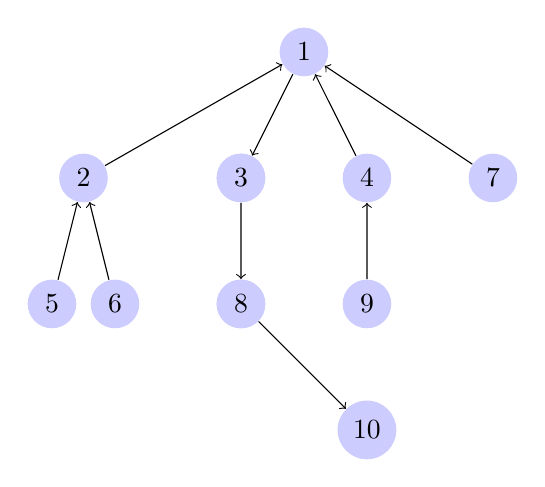
\begin{tikzpicture}
  [scale=.8,auto=left,every node/.style={circle,fill=blue!20}]
 \tikzset{EdgeStyle/.style={->}}
  \node (n1) at (5,8) {1};
 \node (n2) at (1.5,6)  {2};
  \node (n3) at (4,6)  {3};
 \node (n4) at (6,6) {4};
  \node (n5) at (1,4)  {5};
  \node (n6) at (2,4)  {6};
  \node (n7) at (8,6)  {7};
  \node (n8) at (4,4)  {8};
 \node (n9) at (6,4)  {9};
 \node (n10) at (6,2) {10};
  \node (n3) at (4,6)  {3};
  \node (n8) at (4,4)  {8};

 \foreach \from/\to in {n5/n2,n6/n2,n2/n1,n8/n10,n3/n8,n1/n3,n9/n4,n4/n1,n7/n1}
    \draw[->] (\from) -- (\to);

\end{tikzpicture}
\caption{}\label{fig:2}
\end{centering}
\end{figure}
\end{ex}


\subsection{Increasing Pr\"{u}fer Sequences}\label{sec:it}
\begin{defn}[Increasing Pr\"{u}fer sequence]
Given a Pr\"{u}fer sequence, $P_{n}$, we can always build $B_{n}$ as described in Section \ref{sec:itr}.  Let $C_{n} = (c[1],c[2],\dots,c[n-2])$ be the sequence defined componentwise by $c[i] = b[i] - a[i]$ for $i = 1,2,3,\dots,n-2$. if $C_{n}$ satisfies:
\[  \left\{
  \begin{array}{l l}
    c[i] < 0 & \quad \text{if $i \in E$}\\
    c[i] > 0  & \quad \text{otherwise}
  \end{array} \right.\]
and $n \notin P_{n}$ then we say that $P_{n}$ is an \emph{increasing Pr\"{u}fer sequence}.  
\end{defn}

This section culminates in Theorem \ref{lem:5} we will prove that if $P_{n}$ is an increasing Pr\"{u}fer sequence then $P_{n}$ corresponds to an increasing tree. %To do this we will show that for Pr\"{u}fer sequences satisfying this condition $G_{t}$ is built by adding the edge $(a[t-1],b[t-1])$ to $G_{t-1}$ and we will show that a tree built in this way must be an increasing tree.

{\bfseries Throughout the remainder of this section we assume that $P_{n}$ is an increasing Pr\"{u}fer sequence.}  

\begin{lem}\label{lem:0}
If $a[i] \in P_{n}[1 : e_{1} - 1]$ then the vertices with label $a[i]$ are adjacent to vertices with label $b[i]$.

\end{lem}
   
\begin{proof}[Proof of Lemma \ref{lem:0}]
Consider $P_{n}[1 : e_{1} - 1]$.  If $e_{1} = 1$ then there is nothing to do, so assume $e_{1} >1$. Then the Pr\"{u}fer process dictates that the vertex labelled $a[1]$ is connected to the lowest leaf which must be $b[1]$ since $b[1]  = \min L$.  Let $j$ be the smallest value such that $a[j]$ is final.  Then $L_{1} = L_{0} \backslash \{b[1]\}$ and $b[2] = \min L_{1}$ so the vertex labelled $a[2]$ is joined to $b[2]$.  Similarly the vertex $a[3]$ is connected to $b[3]$ until vertex $a[j]$ which is attached to $b[j]$.  Since $a[j]$ is final $a[j] \in L_{j+1}$.  If $j \in E$ then we're done so assume $j \notin E$. By the condition on $C_{n}$, $a[j]<b[j] = \min L_{j}$ so $a[j]$ is not just available it is minimal ($\min L_{j+1} = a[j]$).  Therefore at time  $j+1$ the edge $(a[j+1],a[j])$ is added to make $G_{j+1}$. By the definition of $B_{n}$ this means that $a[j+1]$ is adjacent to $b[j+1]$.  
\end{proof}

If $|E| \geq 2$ then recall that we recursively defined $m_{i} = \min P_{n}[e_{i-1}:n-2]$ for $i = 2,3\dots,n-2$.  For simplicity we define  $P_{n}' = P_{n}[e_{1}:n-2] $ and $P_{n}'' = P_{n}[e_{1} + 1:n-2]$. %We also define $E_{> v} = \{e \in E | e > v\}$.  %Put in some discussion here.

Given any graph $G_{n}$ on $n \geq 2$ vertices the number of vertices $v \in V(G)$ such that $\deg(v) = 1$ is at least 2.  In particular $|L| \geq 2$. We can think of $L_{i}$ as the set of leaves of (not necessarily connected) subgraphs of $T_{n}$ for $i = 1,2,\dots n-2$ so $|L_{i}| \geq 2$ for $i = 1,2,\dots n-2$.  We know that $|L_{n-1}|$ = 2. We also know that  $a[n-2] \in L_{n-1}$ and $\max \{P_{n}[1:n-3], L\} \in L_{n-1}$.  Since we assumed that $n \notin P_{n}$ it must be the case that $n \in L_{n-1}$.  

\begin{lem}\label{lem:1}
Let $|E| \geq 1$ and $e_{1} < n-2$ then there does not exist a vertex $v \in L_{e_{1} + 1}$ such that $v < m_{2}$.     
%Let $P_{n}' = P_{n}[\Pos_{m_{1}X_{m_{1}}}+1 : n-2]$ and $P_{n}'' = P_{n[\Pos_{mX_{m}}+2} : n-2]$.  Let $m_{1} = \min P_{n}$ and $m_{2} = \min P_{n}'$ and $Pos_{m_{1}X_{m_{1}}} < n-4$.  There does not exist a vertex $v<m_{2}$ attached to $a[i] \in P_{n}''$.    
\end{lem}

\begin{proof}
Let $Y_{1} = a[e_{1} + 1]$.  Assume that there exists a vertex labelled $v <m_{2}$ that is attached to some $a[i] \in P_{n}''$. In the language of the Pr\"{u}fer process $v$ must become available to be chosen before at time $e_{1} + 1$.  More precisely $v \in L_{e_{1} + 1}$.  

By the Pr\"{u}fer process $Y_{1}$ is attached to $ v' = \min L_{e_{1} + 1} \leq v$.

\begin{case}[$e_{1}$ is final]
Let $m > e_{1}$ be the least integer such that $a[m]$ is not final. By Lemma \ref{lem:0} $a[i]$ is adjacent to $b[i]$ for $i = 1,2,\dots e_{1}-1$.  Therefore $b[m+1]  = v' \leq v < m_{2}$ this contradicts $C_{n}$ so there does not exist such an $m$.  

Therefore either every $a[i] \in P_{n}'$ is final.  If this is the case then by $C_{n}$: $a[e_{1}] < a[e_{1} + 1] < \dots <a[n-2] < n$ and there cannot be a path between $v'$  and 1.
\end{case}
\begin{case}[$e_{1}$ is not final]
By Lemma \ref{lem:0} $a[i]$ is adjacent to $b[i]$ for $i = 1,2,\dots e_{1}-1$ therefore $b[e_{1}+1] = v' < Y_{1}$ contradicting $C_{n}$.  
 \end{case}
\end{proof}
\begin{lem}\label{lem:2}
 Let $P_{n}$ be defined as in Lemma \ref{lem:1}.  Then $e_{1} = m_{2}$.
\end{lem}
\begin{proof}
 Assume for a contradiction that $e_{1} \neq m_{2}$.  

By Lemma \ref{lem:0} all vertices adjacent to $m_{2}$ which were joined to $a[i]$ for $i = 1,2,3,\dots,e_{1}$ have higher labels than $m_{2}$.  These vertices are further only attached to vertices with labels higher than $m_{2}$ in addition to the edges joining them to these vertices etc..   By Lemma \ref{lem:1} every $m_{2} \in P_{n}'$ is adjacent to some vertex with a higher label. Any of these vertices must be joined to vertices with label larger than $m_{2}$ by the same argument.  Therefore there does not exist a path from $m_{1}$ to $m_{2}$.  This cannot be the case since a Pr\"{u}fer sequence always gives rise to a tree. Therefore $m_{2} = Y_{1}$.      
\end{proof}

%put in some explanation

\begin{cor}\label{cor:1}
 Every Pr\"{u}fer position corresponds to exactly one distinct Pr\"{u}fer entry.  
\end{cor}

\begin{lem}\label{lem:7}
Assume $n >3$, if $e_{1} = n-2$ or $E = \emptyset$ then vertices with label $a[i]$ are adjacent to vertices with label $b[i]$ for $i = 1,2,3,\dots,n-2$.   
%If $m_{1} = 2$, then $a[1]$ is not final, $n>4$ and if $\Pos_{m_{1}X_{m_{1}}} = n-3,n-2$ then vertex $a[i]$ is adjacent to $b[i]$ in $T_{n}$ for all $i$.   
\end{lem}

\begin{proof}
By Lemma \ref{lem:0} vertex $a[i]$ is adjacent to vertex $b[i]$ for $i = 1,2,\dots,\Pos_{1X_{1}}$.  
\begin{itemize}
\item[(i)]
If $E = \emptyset$ then, by Lemma \ref{lem:0} there is nothing to check.   
\item[(ii)]
If $e_{1} = n-2$ then $a[n-3] = m_1$. If $m_1 = 1$ then $ 1 = \min L_{n-2}$ and $1  = b[n-2]$ as required.  If $m_1 = 2$  then 1 must have been attached to $a[1]$, since $n>3$ this is not the case.  
\end{itemize} 
\end{proof}

\begin{lem}
 Every vertex $a[i]$ is attached via an edge to $b[i]$ in $T_{n}$.  
\end{lem}
\begin{proof}
 By Lemma \ref{lem:7} we're done if $e_{1} = n-2$ or $E = \emptyset$ so assume that $E \geq \emptyset$ and $e_1 \neq n-2$.
 
 By Lemma \ref{lem:0} all $a[i] \in P_{n}[1:e_1 - 1]$ are attached via an edge to vertices $b[i]$.  So $a[e_1]$ must be attached to vertex labelled 1 which is $b[e_1]$.  
 
 Using a similar argument to Lemma \ref{lem:0} the subsequent $a[i]$ are attached to $b[i]$ until $a[\Pos_{m_{2},X_{m_{2}}}]$ but by Lemma \ref{lem:2} $m_{2} = e_{1}$.  So we can use the same argument as Lemma \ref{lem:2} to say that $e_{2}$ is attached to $b[e_2]$ as required.  Therefore if $P_{n}$ is a Pr\"{u}fer sequence with the condition $C_{n}$ then at time $i$ we construct $G_{i}$ by adding $(a[i-1],b[i-1])$ to $G_{i-1}$. 
 
 \end{proof}


\begin{lem}\label{lem:4}
 If $b[i] = \min L_{i}$ and $E \neq \emptyset$ then $a[n-2]$ is an exceptional Pr\"{u}fer entry.
\end{lem}

Note that if $b[i] = \min L_{i}$ then at time $i$ the vertex labelled $a[i]$ is attached via an edge to vertex labelled $b[i]$. 

\begin{proof}[Proof of \ref{lem:4}]
Since $E \neq \emptyset$ there exists $e_{1} \in E$.  If $e_{1} = n-2$ the we are  done.  If $e_{1} \neq n-2$ then there exists some $m_{2} = \min P_{n}[e_{1}:n-2]$ and $e_{2} = Pos_{m_{2},X_{m_{2}}+1}$.  Again if $e_{2} = n-2$ we are done.  After enough iterations of this process it must be the case that either $e_{i} = n-2$ or  $a[n-2] = a[n-3] = \dots a[n-m]$ and $e_{i} = a[n-m]$ in either case $a[n-2]$ is an exceptional Pr\"{u}fer entry. 
\end{proof}



%\begin{lem}\label{lem:6}
% If $b[i] = \min L_{i}$ and $E \neq \emptyset$ then $n \notin P_{n}$.
%\end{lem}
%\begin{proof}
%Assume, for a contradiction that $n \in P_{n}$.  Since $|L_{i}|\geq 2$  for $i = 0,1,2,\dots,n-2$ and $a[i]$ is attached to $\min L_{i}$ this means that $\Pos_{nX_{n}} \neq m$ where $m = 1,2,\dots,n-3$. Therefore $n$ is an exceptional Pr\"{u}fer entry.  By Corrolary \ref{cor:1} exactly one ocurrence of $n$ must be exceptional so $P_{n} = (\;,\;,dots,n)$.  

%We know that $|L_{n-1}|$ = 2. Since $a[n-2] \in L_{n-1}$ and $\max \{P_{n}[1:n-3], L\} \in L_{n-1}$.  Since we know that $a[n-2] = n$ it must be the case that $L_{n-1} = \{n,n-1\}$.  

%If $\Pos_{nX_{n}} = n$ then $\dots$. 
%\end{proof}

\begin{thm}\label{lem:5}
If $P_{n}$ adheres to condition $C_{n}$ then $P_{n}$ corresponds to a random recursive tree.  
%$b[i] = \min L_{i}$ and $m_{1} = 1$ then $P_{n}$ corresponds to an increasing tree.  
\end{thm}

\begin{proof}
Consider any $v \in P_{n}$ that is not an exceptional Pr\"{u}fer entry then $v$ occurs $X_{v}$ times in $P_{n}$.  If $v \neq m_{1}$ this corresponds to $X_{v}$ edges with  $v$ as an endpoint such that the other endpoints are vertices with higher labels than $v$ (in particular these vertices are $b[\Pos_{v,1}],b[\Pos_{v,2}],\dots,b[Pos_{v,X_{v}}]$).  By Lemma \ref{lem:4} $v$ is not in position $n-2$ so $v$ is also attached to one vertex with a lower vertex: $a[Pos_{v,X_{v}} + 1]$. If $m_{1} = 1$ then we do not need to worry since for an increasing tree only the \emph{non-root} vertices are required to be attached to precisely one vertex with higher label. If $m_{1} = 2$ then $m_{1}$ is exceptional.       
 
If $v$ is an exceptional Pr\"{u}fer entry then $v$ occurs $X_{v}$ times in $P_{n}$ which, by Corollary \ref{cor:1}, corresponds to $X_{v} - 1$ edges adjacent to $v$ such that the adjacent vertices have a higher label than $v$ and 1 edge adjacent to a vertex with a lower label. 

If $\Pos_{v,X_{v}} \neq n-2$ then $v$ is also attached to another vertex with higher label.  If the final $a[\Pos_{v,X_{v}}]$ is in position $n-2$ then, by the discussion before Lemma \ref{lem:1} $v$ is attached to vertex $n$ and clearly $n>v$ .  Therefore all vertices other than 1 are attached to exactly 1 vertex with lower label than themselves so $T_{n}$ is an increasing tree.     
\end{proof}










%do 1 as a leaf etc.  

%\begin{cor}
%Vertices labelled $a[i]$ are always connected to vertices labelled $b[i]$.  
%\end{cor}



%\subsection{To do List}
%\begin{itemize}
%\item[(i)]Prove the above Lemmas for the case $a[1]$ is final and $m_{1} = 2$

%\item[(ii)]Prove that we get an increasing tree if $a[i]$ is connected to $b[i]$ and $m_{1} = 2$.  

%\item[(iii)]Prove that $a[i]$ is always connected to $b[i]$ if $\Pos_{m_{1},X_{m_{1}}} = n-4.$  


%\end{itemize}

\subsection{Further Directions}\label{sec:fd}
Consider the set of  RRTs on  $n$ vertices: $\mathcal{T}_{n}$.  For each tree $T_{n} \in \mathcal{T}$ if we send every label $i$ to $n - i$ then we form a new set of trees $\tilde{\mathcal{T}}_{n}$.  

The allowable Pr\"{u}fer sequences are $P_{n} = (a[1],a[2],\dots,a[n-2])$ such that $a[i] \in \{2,3,\dots,n-i\}$.  Clearly then there are $n-1!$ possible such Pr\"{u}fer sequences.   

Let $T_{n}$ be a tree chosen at random from the set of $n^{n-2}$ labeled trees.  Let $L_{n}$ be the number of leaves of $T_{n}$, Renyi \cite{Renyi} proved that almost surely:
\begin{align}
 E(L_{n}) & ~ \frac{n}{e} \\
 var(L_{n}) & ~ \frac{(e - 2)n}{e^{2}}
\end{align}
Renyi's proof of these theorems relies upon the Pr\"{u}fer correspondence discussed here.  Our correspondence between increasing Pr\"{u}fer sequences and increasing trees may yield similar theorems for increasing trees.  

\section{Counting Leaves}
Let $T(n,k)$ be the number of increasing trees on $n$ vertices with exactly $k$ leaves then $T(n,k) >0$ if and only if $1 < k < n$. Given some increasing tree $T_{n}$ with $l_{n}$ leaves we can build $n$ new trees by attaching a vertex labeled $n+1$ via an edge to any $n \in V(T_{n})$. The total number of nonisomorphic increasing trees on $n$ vertices is $n-1!$ and since each tree must have some number of leaves we form the following relation:
\begin{equation}\label{eq:i}
 \sum_{k=2}^{n-1}T(n,k) = (n-1)!
\end{equation}


Let $l_{n+1}$ be the number of leaves of any tree $T_{n+1}$ built from $T_{n}$ in the way that we have described, then:
\[  l_{n+1} = \left\{ 
  \begin{array}{l l}
    l_{n}  & \quad \text{if $n+1$ is attached to a leaf}\\
    l_{n} + 1 & \quad \text{otherwise}
  \end{array} \right.\]
Therefore we can recursively define $T(n,k)$.
\begin{ex}
 \begin{align*}
  T(6,5) &= T(5,4) \\
  T(6,4) &= 4T(5,4) + 2T(5,3)\\
  T(6,3) &= 3T(5,3) + 3T(5,2)\\
  T(6,2) &= 2T(5,2)
 \end{align*}

\end{ex}
In general if $ 1< k< n$ then: 
\begin{equation}\label{eq:f}  
T(n,k)= \left\{ 
  \begin{array}{l l l}
    T(n-1,n-2)  & \quad \text{if   $k = n-1$}\\
    kT(n-1,k) + (n-k)T(n-1,k-1) & \quad \text{if   } 2<k<n-1 \\
    2T(n-1,2) & \quad \text{if   }k = 2
   \end{array} \right.
\end{equation}
    
Therefore $T(n,n-1 )  = 2$ for $n >2$.
Similarly we can see by induction that $T(n,2) = 2^{n-2}$.

Let $\mu_{n}$ be the expected proportion of vertices of an increasing tree, $T_{n}$, with degree 1. In addition, let $\nu_{n}$ be the expected number of vertices that are leaves for an increasing tree on $n$ leaves.  
\begin{equation}\label{eq:g}
 \nu_n  = \frac{1}{n-1!}\sum_{k=2}^{k = n-1} kT(n,k) 
\end{equation}

 
We can write that $\mu_{n} = \frac{\nu_n}{n}$.

%It is known that the almost surely $lim_{n \rightarrow \infty}\mu_{n} = \frac{1}{2}$ \cite[Janson} however the proof that Janson gives relies on generalised Polya urn techniques.  We will give a more elementary proof here.  %Will we?????? 

Notice that the recurrence relation for Equation \ref{eq:f} also holds for stirling numbers of the second kind.   

By combining equation \ref{eq:f} with equation \ref{eq:g} and simple manipulation of summations we find that

\begin{align}\label{eq:k}
 \mu_{n} &= \frac{1}{n!}\left( T(n-1,n-2) + 2T(n-1,2) + \sum_{k=3}^{n-2}k\left( kT(n-1,k) + (n-k)T(n-1,k-1)\right)\right) \\
 &= \frac{1}{n!}\left( \sum_{k=2}^{n-2}k^{2}T(n-1,k) + \sum_{k=3}^{n-1}\left(k(n-k)T(n-1,k-1)\right)\right) \\
 &= \frac{1}{n!}\left( \sum_{k=2}^{n-2}k^{2}T(n-1,k) + \sum_{k=2}^{n-2}(k+1)(n-(k + 1))T(n-1,k)\right) \\
 \end{align}

The two sums in equation \ref{eq:k} can be combined since they sum between the same limits (2 and $n-2$) and involve $T(n-1,k)$.  In order to determine the asymptotic value of $\mu_{n}$ we wish to find a simple recurrence relation.  
 Pr\"{u}fer
\begin{align*}\label{eq:j}
 \mu_{n} &= \frac{1}{n!}\left( \sum_{k=2}^{n-2}knT(n-1,k) + \sum_{k=2}^{n-2}(n-1)T(n-1,k) - \sum_{k=2}^{n-2}2kT(n-1,k) \right) \\
  &=  \mu_{n-1} + \frac{1}{n} -  \frac{2\mu_{n-1}}{n}  \\
\end{align*}
Where the last equality above used equation \ref{eq:i}.  Therefore in the limit as $n \rightarrow \infty$ $\mu_{n} \rightarrow \frac{1}{2}$ as we expected.   

\section{Shaving random recursive trees}

Let $T_n$ be a RRT. We say that the induced subtree $T^s_n$ such that $V(T^s_n) = \{ v \in V(T_n) : \deg(v) > 1 \}$ is $T_n$ \emph{shaved}. In this section we produce a simple algorithm for deducing the $\p$ sequence of  $V(T^s_n)$. 

Let $P_n = (a[1],a[2],\dots,a[n-2])$ be the $\p$ sequence associated with the random recursive tree $T_n$ on $n$ vertices built in the way described in Section \ref{sec:fd}.  Recall that we have built $P_n$ in such a way that $a[i]$ is the parent of vertex $i + 2$ for $i = 3,4,\dots,n$ and that the set $L_n = \mathbb{N}_n / P_n$ corresponds to the leaves of $T_n$.

We denote the $\p$ sequence corrosponding to $T^s_n$ by 
\[P_n^s = (a'[1],a'[2],\dots,a'[m])\]
where $m = n - |L_n|$.  Loosely speaking we will build $ P_n^s$ by removing entries from $P_n$. Let $R$  be the set of removed vertices from $P_n$. An algorithm which describes this process is as follows:   

\begin{itemize}
 \item[(i)] Let $R$  be the set of removed vertices from $P_n$ and initially  $R  = \emptyset$.
 \item[(ii)] For every $l \in L_n$ we set $a[l - 2] \in R$.
 \item[(iii)] Let the quotient $ Q = P_n / R$ be the sequence of vertices in $P_n$ and not in $R$.  If we write $Q = (a'[1],a'[2],\dots,a'[m])$ then $a'[1]$ is the first entry in $P_n$ that is not in $R$, $a'[2]$ is the second entry in $P_n$ that is not in $R$ and so on. Then $Q =  P_n^s$
\end{itemize}

\begin{remk}
 The shaved RRT, $T^s_n$, is \emph{not} itself a random recursive tree since the vertices' labels need not be consecutive integers (or even start at 1), however it is relatively straight forward to produce a RRT isomorphic to $T^s_n$. Since $|V(T^s_n)| =  m$ is finite we can order $V(T^s_n)$ from lowest to highest so let $f: V(T^s_n) \rightarrow \mathbb{N}_m$ take the vertex with the lowest label to 1, the second lowest label to 2 and so on.  We call the RRT built in the way described the \emph{reduced RRT} and denote it by $\tilde{T}^s_n$ and the corrosponding $\p$ sequence is denoted by $\tilde{P}_n^s = (\tilde{a}'[1],\tilde{a}'[2],\dots,\tilde{a}'[m])$.
 \end{remk}                            

\begin{ques} Does there exists a $(1,j)$-star in $T^s_n$ which permutes $(1,k)$-stars in $T_n$?
 
\end{ques}
 We have not yet built the appropriate tree to answer this question. We need to classify the leaves of $T^s_n$ by the relevant $(1,k)$-star that has been shaved off.  Let $\m(i)$ denote the multiplcity of each $i \in P_n$ and colour each $i \in R$ by $m(i)$. So the leaves, $\tilde{L}_n^s$, of $\tilde{T}^s_n$ can be partitioned into classes $C_1,C_2,\dots$ according to their colour. 

Now we can define the \emph{$k$-reduced random recursive forest}, $\tilde{T}^s_{n,k}$ which is built as follows:
\begin{itemize}
 \item[(i)] The set of leaves of  $\tilde{T}^s_{n,k}$ are defined to be  $\tilde{L}_{n,k}^s := C_k$.
 \item[(ii)] Remove every element $\tilde{a}^s_n[i]$ such that $i-2 \notin  C_k$. 
\end{itemize}

We can associate the $\p$ sequence $\tilde{P}_{n,k}^s$ with any $k$-reduced random recursive forest $\tilde{T}^s_{n,k}$.

%ARE There names for these things/ standard notations somewhere unheard of?


\begin{ex}
 %ADD EXAMPLE
\end{ex}

\bibliographystyle{h-physrev3.bst}
\bibliography{urns.bib}

\end{document}










